\section{Approach}
\label{sec:alignmentAlg}
%(mostly along the lines of my presentation for the USCMS workshop because it was time when I was the most active)

%Why align?\\
%How to align?\\
%When align?\\
%How to check that your alignment is good?\\

% DOUBLE CHECK WITH FRANK'S PRESENTATION
% MAKE SURE THERE IS NO PLAGIARISM
The concept of track-based alignment can be illustrated in the example of the alignment of a toy tracker (Fig.~\ref{fig:toyTracker_part1}-\ref{fig:toyTracker_part2}). A charged particle crosses a toy tracker of six flat equidistant modules. Because real geometry of the tracker differs from the ideal one, hits are recorded at the places different from the design ideal places. We record and process a large number of tracks to determine positions and orientations of the modules.

\begin{figure}[htb]
    \begin{center}
        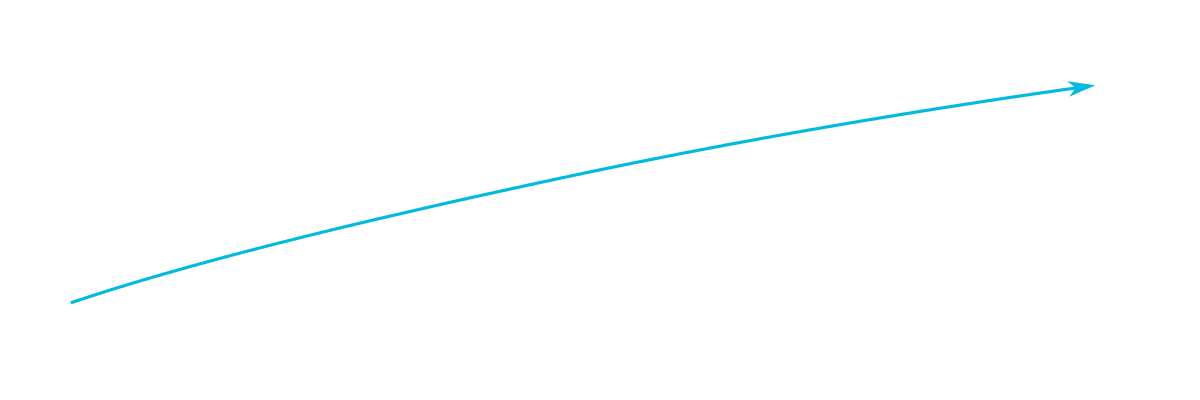
\includegraphics[width=0.45\textwidth]{../figs/Alignment/toyTracker01.png}
        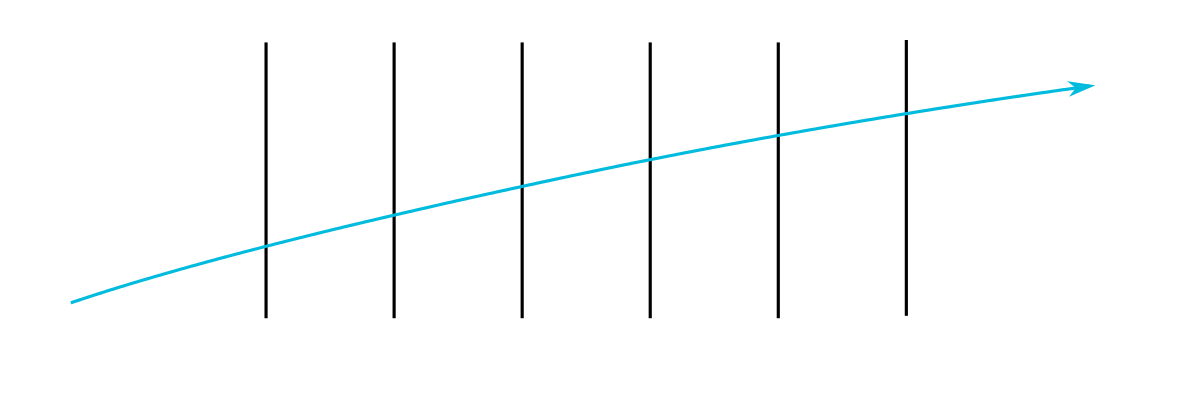
\includegraphics[width=0.45\textwidth]{../figs/Alignment/toyTracker02.png}
        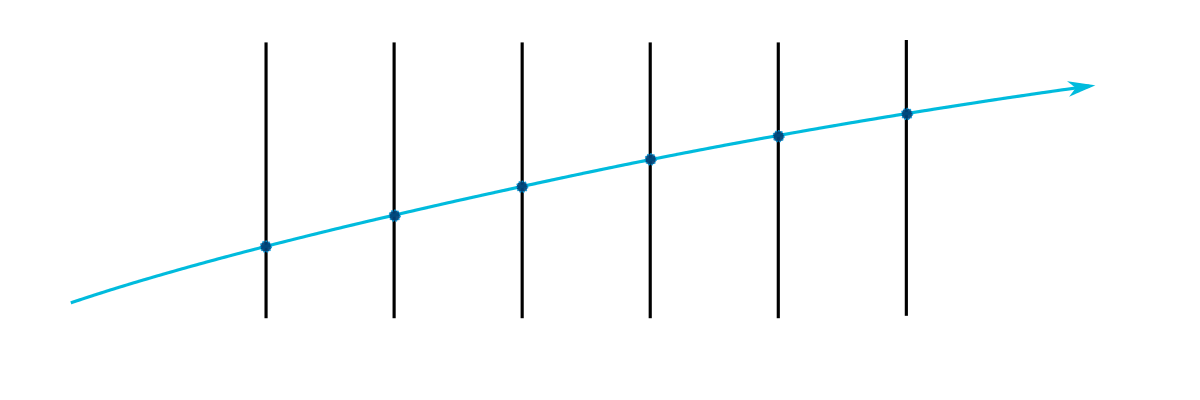
\includegraphics[width=0.45\textwidth]{../figs/Alignment/toyTracker03.png}
        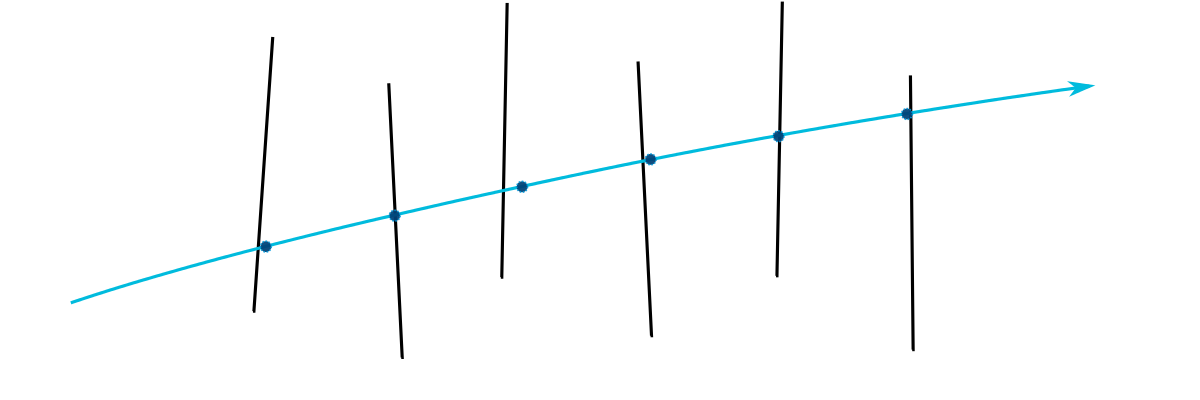
\includegraphics[width=0.45\textwidth]{../figs/Alignment/toyTracker04.png}
        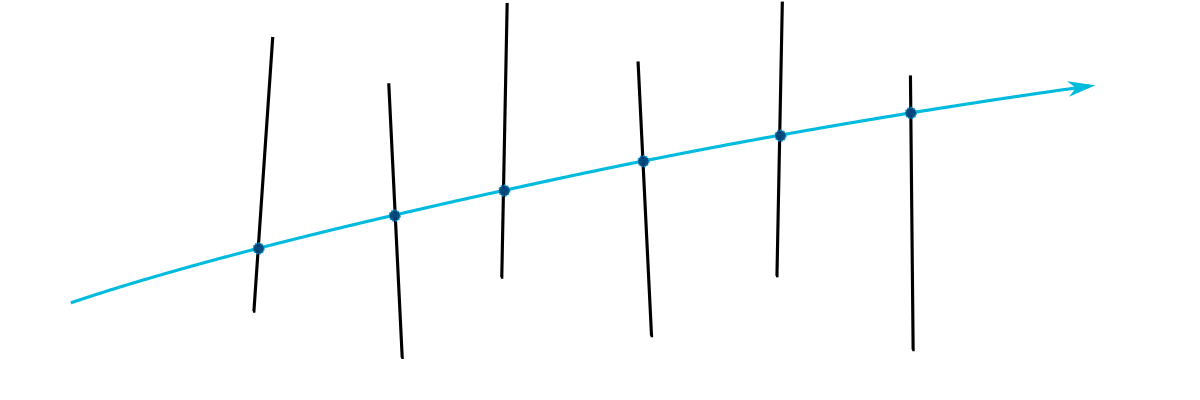
\includegraphics[width=0.45\textwidth]{../figs/Alignment/toyTracker05.png}
        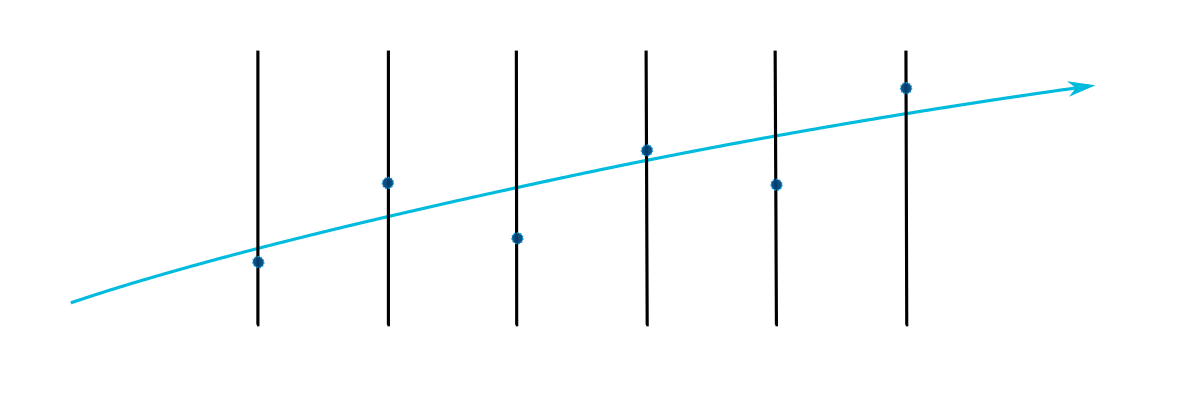
\includegraphics[width=0.45\textwidth]{../figs/Alignment/toyTracker06.png}
    \end{center}
    \caption{The alignment of a toy tracker, part. When a charged particle passing through a detector (top left), it crosses a toy tracker which consists of six flat equidistant modules (top right). If the modules were placed exactly at their designed positions, we would observe the hits exactly at the points where the track crosses modules of ideal geometry (middle left). However, in reality, the positions and tilts of the modules are different from ones suggested by the ideal geometry (middle right). Hits, indeed, are recorded at the places where modules are mounted, not at the design ideal places (bottom left). If we assumed a tracker to be ideal and a track to be smooth, we would see that our hits are off-track (bottom right). Image by Frank Meier.}
    \label{fig:toyTracker_part1}
\end{figure}

\begin{figure}[htb]
    \begin{center}
%        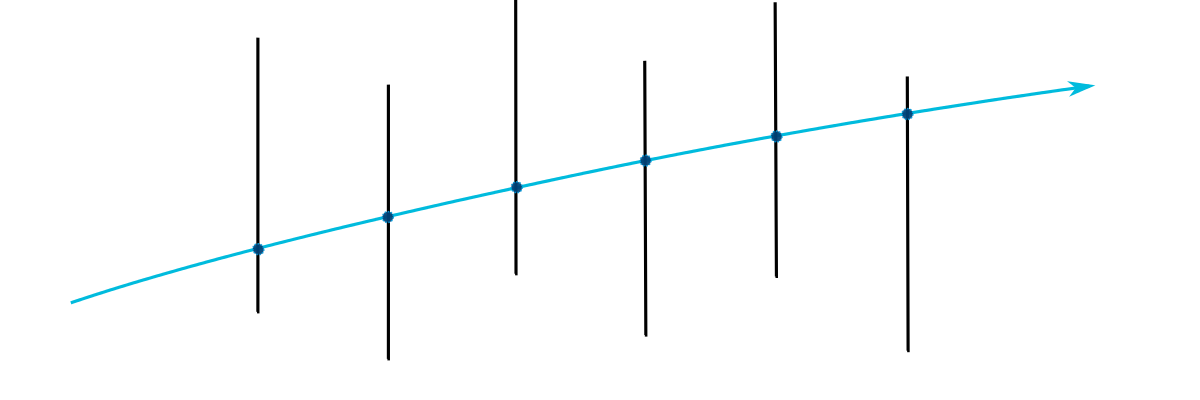
\includegraphics[width=0.45\textwidth]{../figs/Alignment/toyTracker07.png}
%        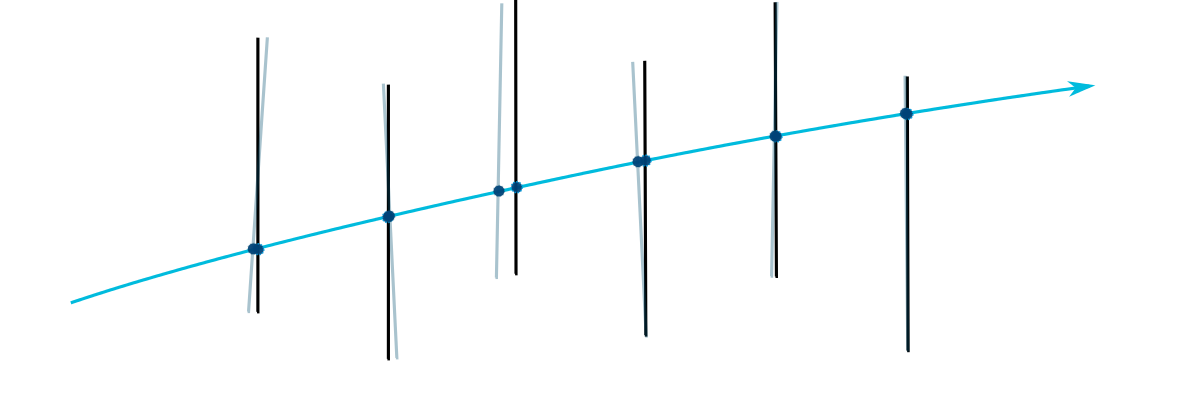
\includegraphics[width=0.45\textwidth]{../figs/Alignment/toyTracker08.png}
%        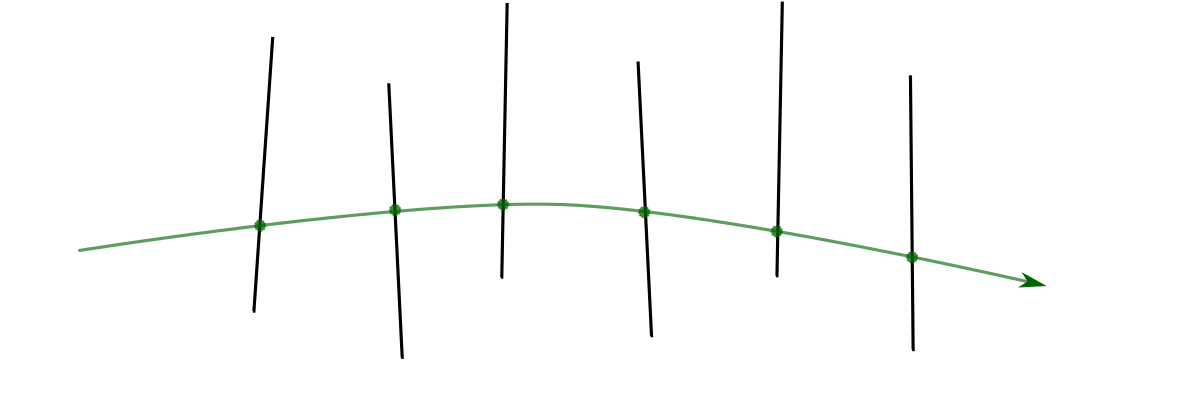
\includegraphics[width=0.45\textwidth]{../figs/Alignment/toyTracker09.png}
%        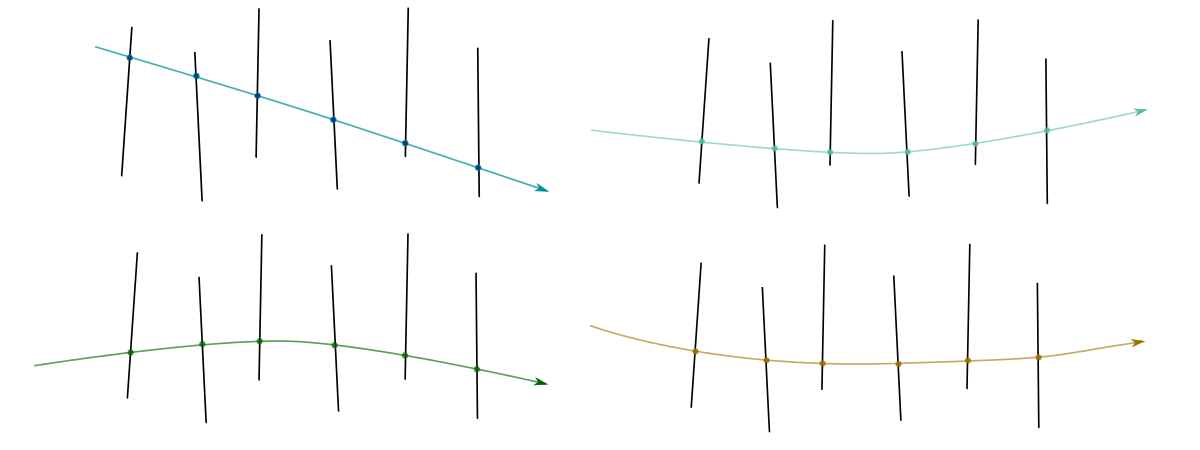
\includegraphics[width=0.45\textwidth]{../figs/Alignment/toyTracker10.png}
        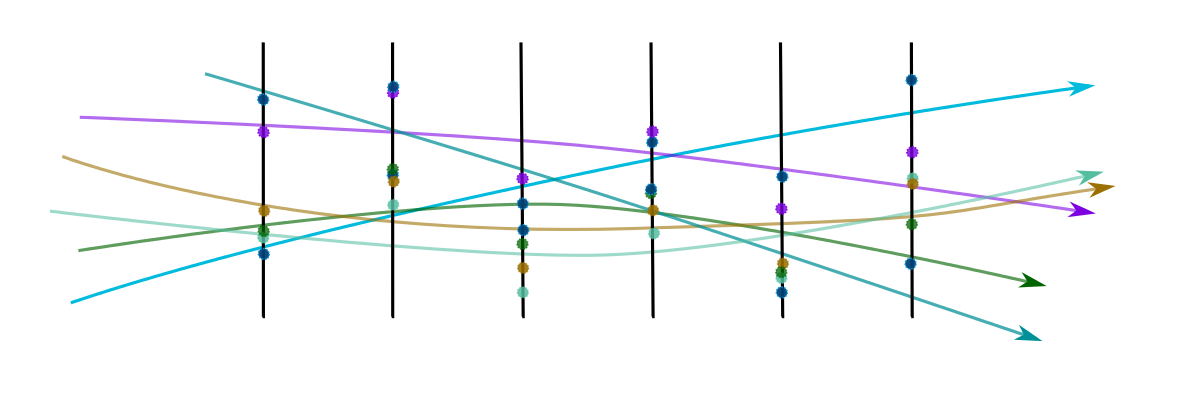
\includegraphics[width=0.45\textwidth]{../figs/Alignment/toyTracker12.png}
        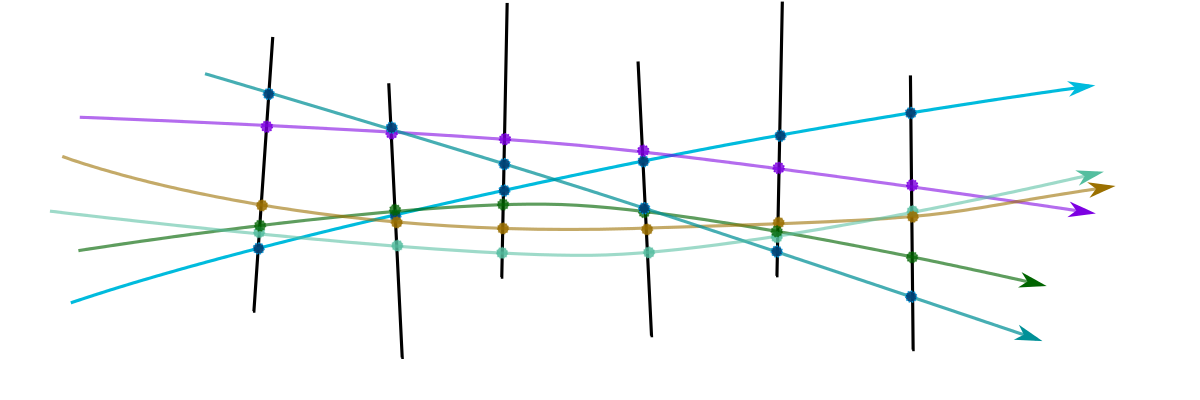
\includegraphics[width=0.45\textwidth]{../figs/Alignment/toyTracker13.png}
    \end{center}
    \caption{The alignment of a toy tracker, part~2. We record a large number of tracks and take into account them all to determine the alignment parameters by minimizing residuals between measured and predicted hits. Image by Frank Meier.}
    \label{fig:toyTracker_part2}
\end{figure}

%The CMS tracker contains 1440 silicon pixel modules in PXB and PXF and 15148 silicon strip modules in TIB, TOB, TID, TEC. 

The tracker alignment problem is a least squares problem. The expression to minimize is the following:

\begin{equation}
  \chi^2(\mathbf{p},\mathbf{q})=\sum_j^{tracks} \sum_i^{hits} \left( {\frac{m_{ij}-f_{ij}(\mathbf{p},\mathbf{q_j})}{\sigma_{ij}}} \right)^2,
\end{equation}

\noindent{where $\mathbf{p}$ are parameters describing the tracker geometry, $\mathbf{q}_j$ are parameters of the $j^{th}$ track, $m_{ij}-f_{ij}$ are distances between the measured hit and a position predicted by the track fit (``residuals''), $\sigma_{ij}$ is the Gaussian error of the measurement.} 

We can align the large substructures with respect to the global CMS coordinate system and individual modules with respect to the coordinate systems of their substructures. The parameters to align large substructures include three coordinates to determine location and three angles to determine orientation of the substracture. At the module level, we align positions and rotations with respect to the positions and angles of the corresponding large structure (Fig.~\ref{fig:alignmentParameters}). Also at the module level, we align for surface deformations which are described by three parameters per sensor (Fig.~\ref{fig:surfaceDeformations}). 

In addition to particles originating from $pp$ collisions of the LHC, CMS also detects muons that originate from interactions of cosmic particles with the Earth's atmosphere. Tracks left by these two types of particles in the tracking system are referred as collision and cosmic tracks respectively. We need both types of tracks for the alignment. %Cosmic tracks pass through the detector vertically and do not allow us to connect different subdetectors to one another. Collision tracks originate from the collision point and go in all directions. However, those tracks which cross TEC are all almost collinear and, therefore, it is difficult to measure $z$-coordinate of TEC modules with collision tracks only.

Two algorithms are used for the alignment of the CMS tracking system: Millepede-II~\cite{ref_MPII_Alg} and HIP~\cite{ref_HIP_Alg}. Millepede-II performs a simultaneous fit of all alignment parameters and all track parameters while HIP performs iterative fits of alignment parameters $\mathbf{p}$ and track parameters $\mathbf{q}_j$.

\begin{figure}[htb]
    \begin{center}
        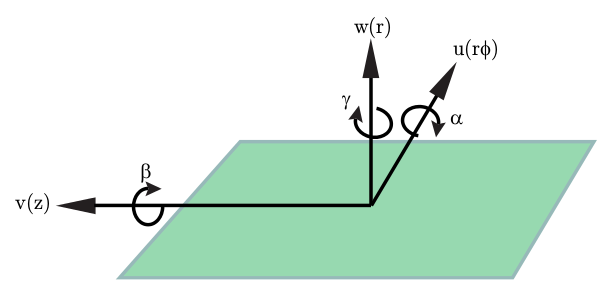
\includegraphics[width=0.70\textwidth]{../figs/Alignment/alignment_strip_coords.png}
    \end{center}
    \caption{Local alignment parameters~\cite{ref_Frank_thesis}.}
    \label{fig:alignmentParameters}
\end{figure}

\begin{figure}[htb]
    \begin{center}
        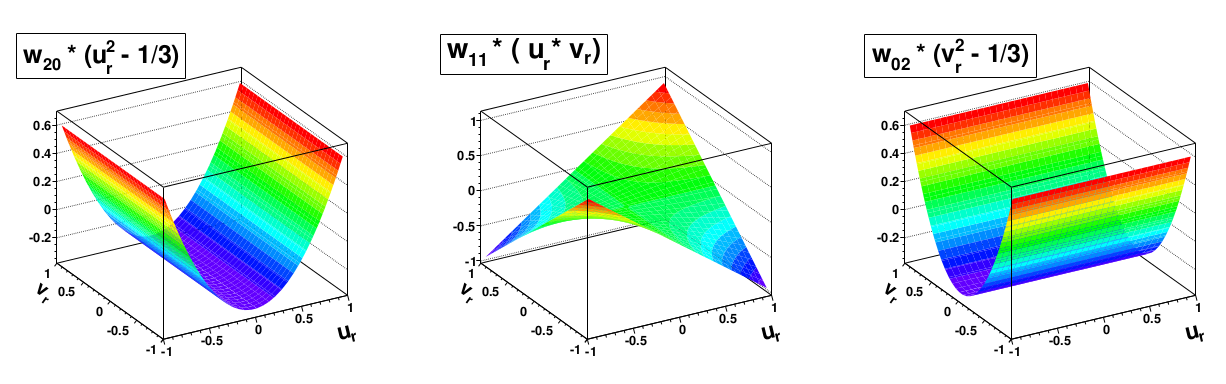
\includegraphics[width=0.90\textwidth]{../figs/Alignment/alignment_surface_deformations.png}
    \end{center}
    \caption{Surface deformations~\cite{ref_Alignment}.}
    \label{fig:surfaceDeformations}
\end{figure}

It is necessary to align a part of the tracking system whenever we suspect a physical change in a location or an orientation of this part. First of all, whenever a part of the CMS tracker is taken out and placed back, we need to realign it. Also whenever a magnet is turned on and off, different parts of the tracking system shift with respect to one another. Pixel half barrels are not screwed firmly, and are moving along each other on rails, therefore, they need to be aligned frequently. Realignment is also necessary when modules are replaced or when the temperature changes. %because it causes the module deformations. 

After the procedure of the tracking system alignment is performed, we validate the results. Chapter~\ref{sec:alignmentResults} discusses various tools of alignment validation using the example of the tracking system alignment based on the~2015 data.   

%\begin{figure}[htb]
%    \begin{center}
%        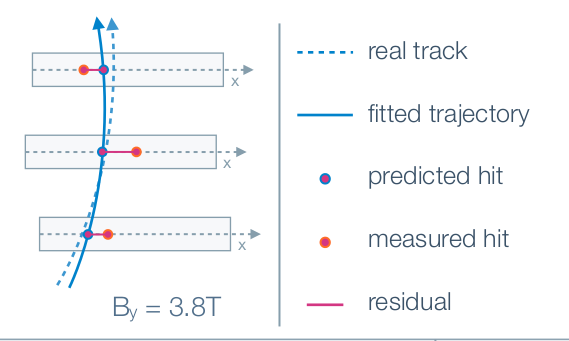
\includegraphics[width=0.70\textwidth]{../figs/Alignment/track.png}
%    \end{center}
%    \caption{Track residuals.}
%    \label{fig:trackAndResiduals}
%\end{figure}

%\begin{figure}[htb]
%  \begin{center}
%    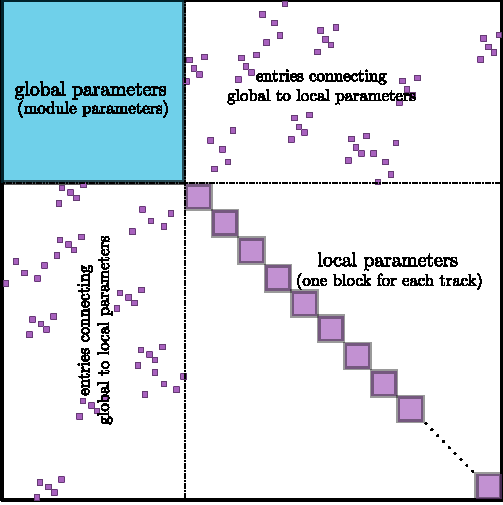
\includegraphics[width=0.70\textwidth]{../figs/Alignment/mpmatrix.pdf}
%  \end{center}
%  \caption{Track residuals.}
%  \label{fig:trackAndResiduals}
%\end{figure}
